\section{Experiments}
\label{appendix:experiments}
In this section, we empirically validate our theoretical framework. A key challenge in evaluating reject-option strategies based on regret is that the calculation of \textit{True Regret} requires access to the true data-generating process $p(y|x, \theta_*)$, which is unknown for real-world datasets.

To address this, we construct a controlled high-dimensional setup that allows us to generate realistic image data while maintaining full access to the ground-truth data-generating process. This enables the exact computation of the Bayes-optimal prediction, the true regret and the true aleatoric uncertainty for every sample, allowing us to benchmark the proposed epistemic reject-option against standard baselines.

\paragraph{Important Note:} This synthetic generation is strictly for validation purposes to verify \Cref{thm:EpistemicRejOpt}. In practice, the proposed Epistemic Reject-Option predictor ($Q_E$) relies only on the learned posterior and does \textbf{not} require knowledge of the ground truth for inference. Only the evaluation of the regret requires access to the data-generating process $p(y|x, \theta_*)$.

\subsection{Experimental Setup}
\paragraph{Data Generation} We define the input distribution $p(x)$ using StyleGAN3 \cite{Karras2021} trained on the Flickr-Faces-HQ Dataset (FFHQ) dataset, which generates high-quality synthetic face images. To define the conditional distribution $p(y|x)$, we create a \textit{Ground-Truth Generator} as follows:
\begin{enumerate}
    \item We train a ViT-B-16 age estimation model on all publicly available age estimation datasets using cross-entropy loss.
    \item We distill the model into a ResNet-50 regression network. This network acts as the oracle: for any input $x$, it outputs a ground-truth mean $\mu_*(x)$ and variance $\sigma^{2}_*(x)$.
    \item Our data generation process is thus defined as $y \mid x \sim \mathcal{N}(\mu_*(x), \sigma_*^{2}(x))$.
\end{enumerate}

For our experiments, we sample a test set of $100,000$ images from $p(x)$. Training sets of varying sizes $m$ are generated by sampling $x \sim p(x)$ and labeling them by sampling a single target $y$ from the $p(y|x)=\mathcal{N}(\mu_*(x), \sigma^{2}_*(x))$.

\paragraph{Models and Training} We employ Bayesian Linear Regression (BLR) as the learning algorithm, implemented as a Gaussian Process with a linear kernel. The learner operates on a fixed feature representation $\phi(x)$ of the input image. We compare three reject-option strategies:
\begin{enumerate}
    \item \textbf{Aleatoric:} Rejects inputs with high irreducible noise using either the true $A_*(x, D)=\sigma_*^2(x)$ or its estimate.
    \item \textbf{Total:} Rejects based on $T_*(x, D)$, the variance of the predictive distribution.
    \item \textbf{Epistemic:} Rejects based on the expected conditional regret $E_*(x, D)$.
\end{enumerate}
    
We employ the Area under the Regret-Coverage Curve and the Area under the Risk-Coverage Curve as our metrics. Risk and regret are calculated using the squared loss.

\subsection{Validation on Well-Specified Models}
We first investigate the setting where the learner is well-specified, meaning the ground-truth function lies within the hypothesis class of the learner. To achieve this, we use the penultimate layer features of the Ground-Truth Generator, the ResNet-50 used to define $p(y|x)$, as the input features $\#\phi(x)\in\mathbb{R}^d$, $d=2048$, for the Bayesian Linear Regressor.

\paragraph{Oracle Aleatoric Variance} Initially, we provide the learner with the true aleatoric variance $\sigma^{2}_*(x)$ to isolate the behavior of the uncertainty estimates. \Cref{fig:oracle_resnet_gp_linear} displays the performance. The proposed Epistemic strategy (red) consistently achieves the lowest Area under Regret Coverage across all sample sizes, empirically confirming that $E_*(x, D)$ is the optimal ranking function for minimizing regret. Conversely the Aleatoric strategy (blue) minimizes Risk. This confirms the theoretical distinction: the Epistemic predictor accepts noisy samples if the model has learned the mean accurately (low regret, high risk), whereas the Aleatoric predictor rejects them.

\begin{figure}[htb]
    \centering
    \begin{minipage}[t]{0.48\linewidth}
        \centering
        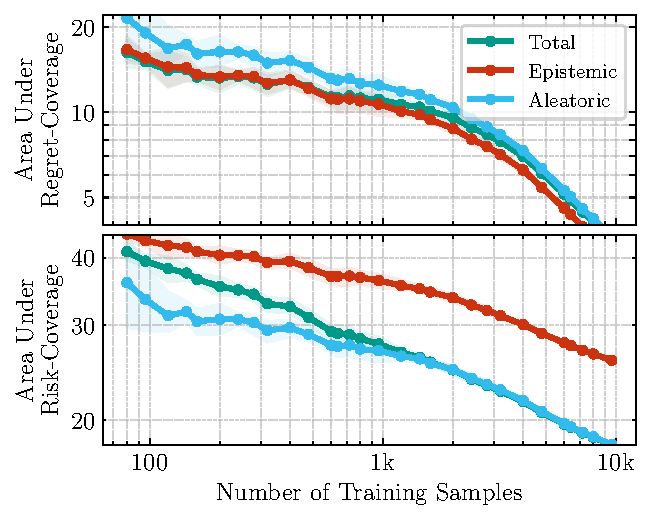
\includegraphics[width=\linewidth]{figures/oracle_resnet_gp_linear.pdf}
        \caption{Performance comparison in the well-specified setting using oracle aleatoric variance. The top row shows the Area Under Regret-Coverage, and the bottom row shows the Area Under Risk-Coverage. As predicted by the theory, the Epistemic reject-option (red) consistently minimizes regret, while the Aleatoric reject-option (blue) minimizes risk. The Total uncertainty (green) acts as an interpolation: in the low-data regime, it is dominated by epistemic uncertainty and follows the red curve; as sample size increases, epistemic uncertainty vanishes, and it converges to the aleatoric behavior (blue curve).}
        \label{fig:oracle_resnet_gp_linear}
    \end{minipage}
    \hfill
    \begin{minipage}[t]{0.48\linewidth}
        \centering
        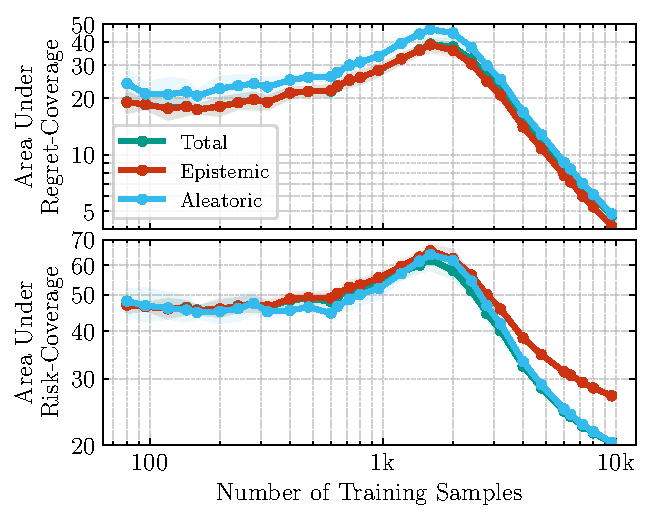
\includegraphics[width=\linewidth]{figures/standard_resnet_gp_linear.pdf}
        \caption{Performance comparison in the well-specified setting using learned aleatoric variance. Here, the noise parameter $\sigma^2$ is estimated via MLE. A characteristic peak in error appears around the interpolation threshold ($|D| \approx d = 2048$). In the under-determined regime ($|D| < 2048$), where the noise estimate often collapses to zero, the Epistemic reject-option (red) remains robust, consistently achieving the lowest regret. This confirms that the posterior variance $E_*(x, D)$ can serve as a proxy for model error even when noise estimation is unstable.}
        \label{fig:resnet_gp_linear}
    \end{minipage}
\end{figure}

\paragraph{Learned Aleatoric Variance} In a realistic setting, $\sigma^{2}_*(x)$ is unknown. We train separate linear layers to estimate the mean $\hat{\mu}(x)$ and noise variance $\hat{\sigma}^2(x)$ via Maximum Likelihood Estimation and use this variance estimate to calibrate the BLR. \Cref{fig:resnet_gp_linear} presents the results. We observe a distinct behavior around $|D| \approx 2048$ samples ($|D| \approx d$). In the under-determined regime ($|D| < d$), the linear model is capable of perfectly interpolating the training data. Consequently, the MLE estimate for the aleatoric variance $\hat{\sigma}^2$ collapses toward zero, effectively leading the learner to treat the data as noiseless. As $|D|$ approaches $d$, the model transitions from interpolation to regression, resulting in the characteristic \textit{double descent} peak in risk and regret due to the ill-conditioning of the covariance matrix. Notably, despite the variance estimate collapsing in the low-data regime and the spectral instability at the interpolation threshold, the Epistemic reject-option maintains the property of minimizing regret. This demonstrates that the posterior variance of the weights $E_*$(x, D) remains a robust signal for model error, even when the aleatoric noise estimate is unreliable.

\subsection{Limitations under Model Misspecification}
We further investigate a \textit{misspecified} setting where the ground-truth function lies outside the hypothesis class. We replicate the experimental setup using FaRL features \cite{Zheng_2022_CVPR}, rendering the true function $\mu_*(x)$ non-linear with respect to the linear Bayesian predictor. In this regime, as $|D| \to \infty$, the parameter posterior concentrates around a single linear approximation. Consequently, the epistemic uncertainty vanishes, yet the regret converges to a non-zero constant corresponding to the approximation error (bias). This reveals a fundamental property: the proposed epistemic reject-option specifically targets \textit{estimation error} (finite data) rather than \textit{approximation error} (limited capacity). Notably, preliminary investigations suggest this behavior is not unique to the linear setting; we observed similar results with Gaussian Processes with RBF kernel and Deep approximations (MC Dropout, Deep Ensembles), highlighting an open challenge for the field.